\documentclass[14pt]{beamer}
\usepackage{beamerthemesplit}
\usetheme{Madrid}
\usefonttheme{serif}
\usepackage{bookman}

\title[SPIN]{Student Project Information Network}
\author[Damini Charvitha Lendi ]{K. Damini Satya \\K. Sri Charvitha\\M. Lendi Vihari}
\institute[BVRITH]{Department of Information Technology and Computer Science\\II Year\\BVRIT Hyderabad}
\begin{document}

\maketitle

\begin{frame}
\frametitle{Problem Statement}
Roughly 500 students, 4 branches, 3 programs
\begin{itemize}
	\item What is happening?
	\item How are we doing?
\end{itemize}
\end{frame}

\begin{frame}
\frametitle{Users}
\begin{itemize}
	\item Students
	\item Management
\end{itemize}
\end{frame}

\begin{frame}
\frametitle{Purpose}
\begin{block}{Students}
	Get notified with technical and non-technical information.
\end{block}
\begin{block}{Management}
	\begin{itemize}
		\item Analyse overall performance of students.
		\item Know details of the programs. 
		\item Know the effectiveness of the programs being conducted.
	\end{itemize}
\end{block}
\end{frame}

\begin{frame}{Application Taxonomy}
	\begin{center}
	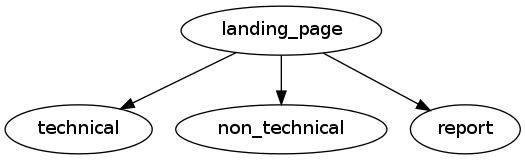
\includegraphics[scale = 0.45]{spin.png}\\
	\end{center}
\end{frame}

\begin{frame}{Application Taxonomy}
	\begin{center}
	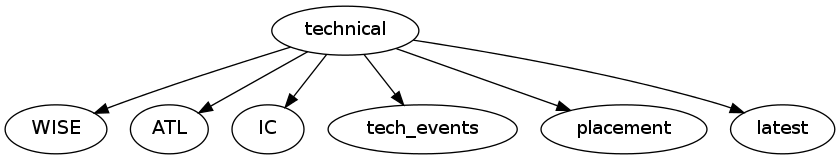
\includegraphics[scale = 0.38]{tech.png}
	\end{center}
\end{frame}

\begin{frame}{Application Taxonomy}
	\begin{center}
	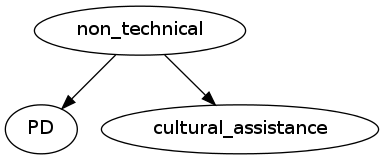
\includegraphics[scale = 0.5]{nontech.png}
	\end{center}
\end{frame}

\begin{frame}{Application Taxonomy}
	\begin{center}
	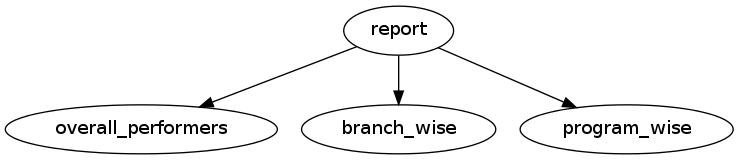
\includegraphics[scale = 0.4]{report.png}
	\end{center}
\end{frame}

\begin{frame}{Administrator}
	\begin{itemize}
		\item Notify about programs.
		\item Publish related content.
		\item Maintain and Manipulate  database.
	\end{itemize}
	\begin{center}
	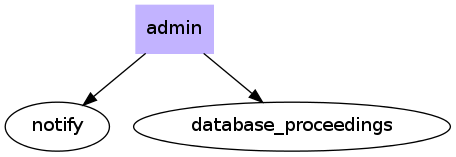
\includegraphics[scale=0.5]{admin.png}
	\end{center}
\end{frame}

\end{document}
